%%%%%%%%%%%%%%%%%%%%%%%%%%%%%%%%%%%%%%%%%
\documentclass[12pt]{article}
% Set the margins to 1 inch
\usepackage[margin=1in]{geometry}
% Line numbers 
\usepackage{graphicx}	
\usepackage{float}

\usepackage{natbib}

% Authors
\usepackage{authblk}
\renewcommand\Affilfont{\itshape\small}

% Double spacing between lines
\usepackage{setspace}
%
\usepackage{titlesec}
\renewcommand{\thesubsection}{\alph{subsection}.\itshape}

\titleformat{\subsection}{\itshape\normalsize}{\thesubsection}{1em}{}
\titlespacing{\subsection}{\parindent}{*2}{\wordsep}      
\renewcommand{\thesubsubsection}{\roman{subsubsection}.\itshape}

\titleformat{\subsubsection}{\itshape\normalsize}{\thesubsubsection}{1em}{}     
 \titlespacing{\subsubsection}{\parindent}{*4}{\wordsep}

\usepackage{color}

\sloppy
\definecolor{lightgray}{gray}{0.5}
\setlength{\parindent}{0pt}


%----------------------------------------------------------------------------------------
%	DOCUMENT INFORMATION
%----------------------------------------------------------------------------------------
\title{Using Diabox \\ Introduction to inverse modeling \\ Physical Oceanography} % Title

\author{Lo\"{\i}c Jullion, Rick Lumpkin \& Kevin Speer} % Author name

\date{\today} % Date for the report

\begin{document}
\maketitle
\thispagestyle{empty} 
\clearpage

% 
% If you wish to include an abstract, uncomment the lines below
% \begin{abstract}
% Abstract text
% \end{abstract}
\tableofcontents
\clearpage

%----------------------------------------------------------------------------------------
%	INTRODUCTION
%----------------------------------------------------------------------------------------

\section{Objective}

Inverse modeling \citep{wunsch96} is a method to estimate the large-scale oceanic circulation by combining observations in a simple theoretical framework in which conservation of mass and other tracers is enforced. A box model solves for unknowns (reference levels for thermal wind, diapycnal fluxes, adjustments to air-sea fluxes) in order to satisfy property conservation constraints in closed boxes.  As the name suggests, a box model consists of one or more boxes, each delineated by coastlines and hydrographic sections. 

Inverse modeling has been widely used to diagnose the global circulation (\textit{e.g.}\cite{Lumpkin:2007tn}; \cite{Ganachaud:2000uo}; \cite{Macdonald:1998vy}; \cite{Talleyetal:2003}), the regional circulation (\textit{e.g.} \cite{Jullion:2010ew,Jullion:2013}) and the transport of biogeochemical tracers \citep{Ganachaud:2002ec,TorresValdes:2013fw}. 

DIABOX is a modification of DOBOX 4.2, a Matlab software package for constructing, inverting and analyzing box inverse models developed at the CSIRO Climate Change Research Program \citep{Morgan94}.  DIABOX development began in 2000, and has continued under NSF funding (PIs R. Lumpkin and K. Speer, Florida State University).  Current development is handled by Rick Lumpkin (Cooperative Institute for Marine and Atmospheric Sciences, Univ. Miami) and Lo\"{\i}c Jullion (FSU). DIABOX adds explicit air-sea transformation for outcropping layers, includes greater automation than in DOBOX for often-repeated steps, collects global choices for hydrographic sections into a single file, solves for unknowns via Gauss-Markov inversion, and fixes several bugs identified in DOBOX 4.2 code.

The objectives of this report are to: 

\begin{description}
\item[First Objective:] Lay out the basic physics and equations underpinning box inverse models. For a thorough presentation of the box inverse model approach, a reader is referred to \cite{wunsch96}. \\

\item[Second Objective:] Introduce the necessary steps to set up a new inverse model and provide a description of the different routines, highlighting the differences with the original DOBOX 4.2 code\\

\end{description}

%----------------------------------------------------------------------------------------
%	SECTION 2: Inverse modelling 101
%----------------------------------------------------------------------------------------

\section{Theory of box inverse modelling}
	\subsection{Conservation and geostrophy}
	
	Consider an oceanic region closed by continents and hydrographic sections and assume the large-scale, steady state circulation is in quasi-geostrophic balance. We write the conservation of any tracer as:

\begin{equation}\label{con_trac}
(\overrightarrow{U}.\nabla)\rho C = \frac{\partial}{\partial
z}\kappa_{v}\frac{\partial(\rho C)}{\partial z} + q(x,y,z),
\end{equation}
with \emph{C} being the tracer concentration, $ \overrightarrow{U}=\left\{
\begin{array}{l}
u\\
v\\
w
\end{array}
 \right\} $, the velocity. $\kappa_{v}$, the vertical diffusivity and \emph{q} a source/sink term. In other words: What goes in the box must somehow get out too as in a steady state, there is no piling up of water in certain basins or drainage in others. Under the quasi-geostrophic assumption, the horizontal velocity \emph{v} can be approximated to the geostrophic velocity  normal to the hydrographic section and it can be calculated from the thermal wind equation: 
\begin{equation} \label{thermal wind}
-f\frac{\partial(\rho v)}{\partial z} = g \frac{\partial
\rho}{\partial x},
\end{equation}
where \emph{f} is the coriolis paremeter (\emph{f} = $2\Omega\sin\varphi$, with $\Omega$, the rotation rate of the earth and $\varphi$, the latitude), $\rho$ is the density of sea water and \emph{g}, the acceleration of gravity. If Equation \ref{thermal wind} is vertically integrated from the surface to a certain level in the ocean along the sections S$_{1}$ and S$_{2}$, one obtains:

\begin{equation} \label{integrated_thermal_wind}
\rho v(x,z) =
\underbrace{-\frac{g}{f}\int^{z}_{z_{0}}\frac{\partial
\rho}{\partial x}dz}_{baroclinic \textrm{ } component} +
\underbrace{\rho b(x,z_{0})}_{barotropic \textrm{ }component}
\equiv (v_{R}+b)\rho,
\end{equation}
with $z_{0}$, the reference level used to integrate Equation \ref{thermal wind} vertically. The baroclinic component, (v$_{R}$), can be perfectly determined from observations of temperature and salinity except for the errors of measurement. The barotropic component $b(x,z_{0})$ however cannot be directly determined from observations but can be approximated based on direct velocity measurements (ADCPs, current meters).
 
We can divide the hydrographic sections closing the box vertically in density layers representing for example the main water masses. Assuming the flow is non-divergent and that the tracer does not have any sink/source in the box, we write equation \ref{con_trac} for a layer delimited by 2 density interfaces \emph{$\gamma_{\jmath}$} and \emph{$\gamma_{\jmath+1}$}:
\begin{equation}\label{int_trac_cons}
\oint_{box}\int_{\gamma_{\jmath}}^{\gamma_{\jmath+1}}(v_{R}+b)\rho C d\gamma dn = \biggl[\int_{A_{\gamma}} \kappa_{v}\frac{\partial(\rho C)}{\partial \gamma} dA \biggr]_{\gamma_{\jmath}}^{\gamma_{\jmath+1}} - \biggl[\int_{A_{\gamma}}w\rho dA \biggr]_{\gamma_{\jmath}}^{\gamma_{\jmath+1}}
\end{equation}
$\oint_{box}$ and $\int_{A_{\gamma}}$ represents the integral along the rim of the box and over the area of an isopycnal layer $\gamma$ in the box interior respectively. \emph{dn} is the direction orthogonal to the hydrographic section, \emph{w} is the diapycnal velocity across an isopycnal. Note that the isopycnal diffusivity is not included explicitly in the model as its inclusion is difficult and the results uncertain \citep{mcintoshandrintoul97}.
 
Equation \ref{int_trac_cons} states that for a tracer C, the convergence/divergence of the lateral fluxes (the left hand side of \ref{int_trac_cons}) is compensated by a vertical fluxes across the layer's interfaces. Following \cite{mcintoshandrintoul97}, we parameterized these vertical fluxes by a diapycnal velocity $\omega^{\star}_{c}$ for each tracer C encompassing the effects of both advective and diffusive processes. Therefore, even if $\omega^{\star}_{c}$ has the dimension of a velocity, it is not equal to the vertical velocity \emph{w} (except when considering volume) as $\omega^{\star}_{c}$. We express  $\omega^{\star}_{c}$ as:

\begin{equation}\label{diap_flux}
\biggl[\int_{A_{\gamma}} \kappa_{v}\frac{\partial(\rho C)}{\partial \gamma} dA \biggr]_{\gamma_{\jmath}}^{\gamma_{\jmath+1}} - \biggl[\int_{A_{\gamma}}w\rho dA \biggr]_{\gamma_{\jmath}}^{\gamma_{\jmath+1}} = [\overline{A}\overline{\rho}\overline{C}\omega_{c}^{\ast}]_{\gamma_{\jmath+1}}- [\overline{A}\overline{\rho}\overline{C}\omega_{c}^{\ast}]_{\gamma_{\jmath}}
\end{equation}
where \emph{A} is the area of the layer interface, \emph{C} is the tracer concentration at the interface and $\omega_{c}^{\ast}$ is the "diapycnal velocity" for \emph{C}. Here, $\overline{(\cdot)}$ denotes the mean value over the layer interface. Therefore, the conservation equation for a given layer in the box is given by:

\begin{equation}\label{inverse_equation}
\oint_{box}\int_{\gamma_{\jmath}}^{\gamma_{\jmath+1}}(v_{R}+b)\rho C d\gamma dn = [\overline{A}\overline{\rho}\overline{C}\omega_{c}^{\ast}]_{\gamma_{\jmath+1}}- [\overline{A}\overline{\rho}\overline{C}\omega_{c}^{\ast}]_{\gamma_{\jmath}}
\end{equation}

Neutral density surfaces \citep{Jackett:1997p370} are usually chosen to divide the ocean vertically in density layers even though other choices of density surfaces can be made, particularly in places where neutral densities have not been defined yet (the Arctic, the Mediterranean Sea, the Red Sea...). The layer interfaces are usually chosen so that the limits of the main water masses present in the box are represented in order to obtain a consistent view of the transport of individual water masses. The conservation statement for any given tracer \emph{C} (Eq. \ref{inverse_equation}) can be written in its discretize form as:
	
\begin{equation}\label{conservation}
\sum_{\imath=1}^{n}\sum_{\jmath=1}^{m}[\delta_{\imath}L_{\imath}D_{\imath \jmath}(V_{\imath\jmath}+b_{\imath})\rho_{\imath\jmath}C_{\imath\jmath}] - [A\overline{\rho C\omega_{c}^{\ast}}]_{\gamma_{\jmath}}^{\gamma_{\jmath+1}}= 0
\end{equation}

$\imath=1 \ldots n$ is the number of station pairs, $\jmath=1 \ldots m$ is the number of layers, $L_{\imath}$ and $D_{\imath\jmath}$ are the distance between stations and layer thickness at each station respectively, $\delta_{i}$ takes the value +1 or -1 depending on whether the transport is into or out of the box. \emph{A} is the area of the layer interface, $\omega_{c}^{\ast}$ is the "diapycnal velocity" for \emph{C}. $\overline{(\cdot)}$ denotes the mean value over the layer interface. 

	Equation \ref{conservation} represents the most basic form of inverse modelling for a given layer in which only the oceanic transport is taken into account. Similar equations can be written for all the layers as well as for the full depth transport to form a system of equations.

	\subsection{Additional terms}
	A strength of inverse modelling is the possibility to add extra terms to the conservation equation in order to improve the representation of additional physical processes. Typically, we also need to account for exchanges of mass, heat and salt (freshwater) between the air, the continent and the Oceans. In polar oceans, the export of mobile sea-ice will play an important role in the freshwater and heat budgets. Finally, one can estimate the contribution of the time-varying circulation (as opposed to the steady-state transport usually given by inverse models). The time-varying circulation will be referred to as \textit{eddy fluxes}. We expand Eq. \ref{conservation} to incorporate sea ice, eddy and air-sea surface fluxes:

\begin{equation}\label{conservation_2}
\sum_{\jmath=1}^{m}\sum_{\imath=1}^{n}[\delta_{\imath}L_{\imath}D_{\imath \jmath}(V_{\imath\jmath}+b_{\imath})\rho_{\imath\jmath}C_{\imath\jmath}] + \nu_{\jmath}(C) - [A\overline{\rho C\omega_{c}^{\ast}}^{\gamma}]_{\gamma_{\jmath}}^{\gamma_{\jmath+1}} + F^{A-S}_{\jmath}(C) + F^{SI}_{\jmath}(C)  = 0 ,
\end{equation}
%\begin{center}
%\begin{eqnarray}\label{seaice}
%\sum_{\imath=1}^{n}[\delta_{\imath}L_{\imath}D_{\imath m}(V_{\imath m}+b_{\imath})\rho_{\imath m}] + \sum_{\imath=1}^{n}[T^{si}_{\imath}] - F_{V}   &=& 0\\
%\sum_{\imath=1}^{n}[\delta_{\imath}L_{\imath}D_{\imath m}(V_{\imath m}+b_{\imath})\rho_{\imath m}S_{\imath m}'] + \sum_{\imath=1}^{n}[v^{si}_{\imath}A^{si}_{\imath}S^{si'}_{\imath}]  &=& 0\\
%\sum_{\imath=1}^{n}[\delta_{\imath}L_{\imath}D_{\imath m}(V_{\imath m}+b_{\imath})\rho_{\imath m} \Theta_{\imath m}'] + \sum_{\imath=1}^{n}[H^{si}_{\imath}]-F_{\Theta} &=& 0
%\end{eqnarray}
%\end{center}

\noindent where $n$ is the number of station pairs; $m$ is the number of layers; $\delta_{i}$ adopts the value +1 or -1 depending on whether flow is directed into or out of the box; $L_{\imath}$ and $D_{\imath\jmath}$ are the distance between successive stations and the layer thickness at each station pair, respectively; V$_{\imath\jmath}$ is the baroclinic velocity at the station pair $i$ and layer $j$; b$_{\imath}$ is the barotropic velocity offset at station pair $i$; $\rho_{\imath\jmath}$ is \textit{in situ} density; $\emph{A}$ is the area of the layer interface within the box; $\omega_{C}^{\ast}$ is the diapycnal velocity for tracer \emph{C} \citep{mcintoshandrintoul97,sloyan00}; $F^{A-S}(C)$ and $F^{SI}(C)$ are the fluxes of tracer \emph{C} associated with air-sea interactions and sea ice, respectively;  $\nu_{\jmath}(C) = \rho_{\jmath}[\overline{v'C'}\overline{h} + \overline{v'h'}\overline{C}]_{\jmath}$ is the eddy-induced flux of tracer \emph{C} for the layer $\jmath$, which consists of advective (the first) and diffusive (the second) components; $\overline{(\cdot)}^{\gamma}$ and $\overline{(\cdot)}$ denote the area-mean operator over a layer interface and the time-mean operator, respectively. The air-sea fluxes and their impact on water mass transformations are described in greater details further down. 

	\subsection{Solving the system}
	
We write a set of equations for the different tracers in a matrix form:
 \begin{equation}\label{matrix_form}
 A\mathbf{X} + \mathbf{n} = 0
 \end{equation}	
 where A is the model matrix containing the coefficients multiplying the unknowns in Eq. \ref{conservation_2} and $\mathbf{X}$ contains the unknowns we wish to quantify. Here $\mathbf{X} = [\omega_{c}^{\ast}, b_{\imath}, \nu_{\jmath}(C), \omega_{c}^{\ast}, F^{A-S}(C) + F^{SI}(C)]$. Typically, Eq. \ref{matrix_form} contains more unknowns than equations and the system is underdertemined, leading to an infinity of solutions satisfying \ref{matrix_form}.

We can introduce an \textit{a priori} solution in  Eq. \ref{matrix_form} based on available observations. We can decompose:
 \begin{equation}\label{unknown1}
\mathbf{X} = \mathbf{X} ^{obs} +\mathbf{X} ^{'} 
 \end{equation}
	
where $\mathbf{X} ^{obs}$ and $\mathbf{X} '$ denote the observed component and adjustment made by the inverse model respectively. Introducing Eq. \ref{unknown1} in Eq. \ref{matrix_form}, we calculate the imbalances in the observation-based estimate of each conservation equation:
 \begin{equation}\label{residual}
 \mathbf{b} = \mathbf{A}\mathbf{X^{obs}},
 \end{equation}
so that we write:
  
 \begin{equation}\label{matrix_form_2}
 A\mathbf{x} + \mathbf{n} = \mathbf{b}
 \end{equation}
$\mathbf{x}$ contains the unknowns, $\mathbf{b}$ contains the \textit{a priori} imbalances and $\mathbf{n}$ is the noise vector which represents the errors and uncertainties associated with the different terms and conservation statements. We now have a set of conservation equations constrained by observations. We can solve Eq. \ref{matrix_form_2} using classical inverse solution (Singular value decomposition or Gauss-Markov estimation). See \cite{wunsch96} for a detailed description of the two methods.
		  	
%----------------------------------------------------------------------------------------
%	SECTION 3: Preprocessing using DIABOX
%----------------------------------------------------------------------------------------
\section{Setting up DIABOX}
After this basic introduction to inverse modeling, we describe now the different steps to build and run an inverse model using the software DIABOX. Running DIABOX requires several steps:

\begin{enumerate}
  \item Preparing the hydrographic sections for use in DIABOX.
  \item Identifying the geometry of the box model.
  \item Constructing the box model in Matlab.
  \item Setting up the matrices and inverting, using DIABOX.
  \item Plotting and interpreting the results.
\end{enumerate}

	\subsection{Installing DIABOX}

Once you have download the tar file, set up the directory where you want. Here we assume the directory is installed in $\sim$/Work/ . The directory is made of several sub-directories and mfiles. A Documentation directory where the PDF of the User guide is found. The directories \verb"main_files" and \verb"mutil" contain the main files for the inverse model. The directory \verb"preproc" contains the files needed for the preprocessing of the hydrographic data. We suggest you add the path to the directories \verb"Diabox_v2.0/main_files" and \verb"Diabox_v2.0/mfiles" to your \textit{pathdef.m} file.

Once the software is installed, you can run the \verb"create_new_inversion.m" file with the path to the directory where you want to do the work. For example:

\begin{tabular}{l}
\verb">>create_new_inversion('~/Work/test_inversion');"\\
\end{tabular}

This will create a directory \verb"test_inversion/" and the corresponding sub-directories. It will also store the path to the directory in the \verb"dir_loc.mat" file and copy different template files. These files are the main files that will need to be updated for each new inversion (2 other possible mfiles that will need to be updated if extra terms are added to the inversion are \verb"getXcol.m" and \verb"updateA_b.m").

	\subsection{Pre-inversion processing}

 		\subsubsection{Preparing the section files for use in DIABOX}

The hydrographic sections need to be converted into Matlab format first. The hydrographic sections are formatted using  \verb"prepctd.m". This program performs several tasks:
\begin{enumerate}
  \item Test to see that a temperature and salinity values exist at every 2db data point within a cast. If not it interpolates to find these values.
  \item Calculates geostrophic velocity between stations to  deepest common depth.
  \item Adds the geostrophic velocity to area beneath deepest common depth using (v=const. ie. dvdz=0). Calculates the area of the bottom triangle. 
  \item Find temperature and salinity values at standard depths. In the upper 500 db this is the actual value property value at the standard depth. Below this it is a 20 db mean centred around standard depth.
  \item Calculates the $\gamma_{n}$ values for the section, using the 2db data. Then finds the temperature, salinity and pressure value for chosen neutral surfaces. The mean pressure between these stations of neutral surfaces is then calculated.  
\end{enumerate}

The results of the pre-processing will be stored in 3 variables, for example in the case of A08: \verb"a08_raw.mat", \verb"a08_ns.mat" and \verb"a08_tria.mat" in the subdirectory:

 \noindent\verb"~/Work/test_inversion/sections/". 

	\subsection{Identifying the box geometry}

We start with a simple 2 box model of the North Atlantic built using 5 sections (Figure \ref{fig1}). An equatorial box closed in the South by A08 (along $11^{\circ}$S) and in the North by A05 (along $24^{\circ}$N). The mid-latitude box is closed by A05 and AR19 near $48^{\circ}$N. The Mediterranean Sea is also closed by a section Between Spain and North Africa (Ar16).

\begin{figure}
\begin{center}
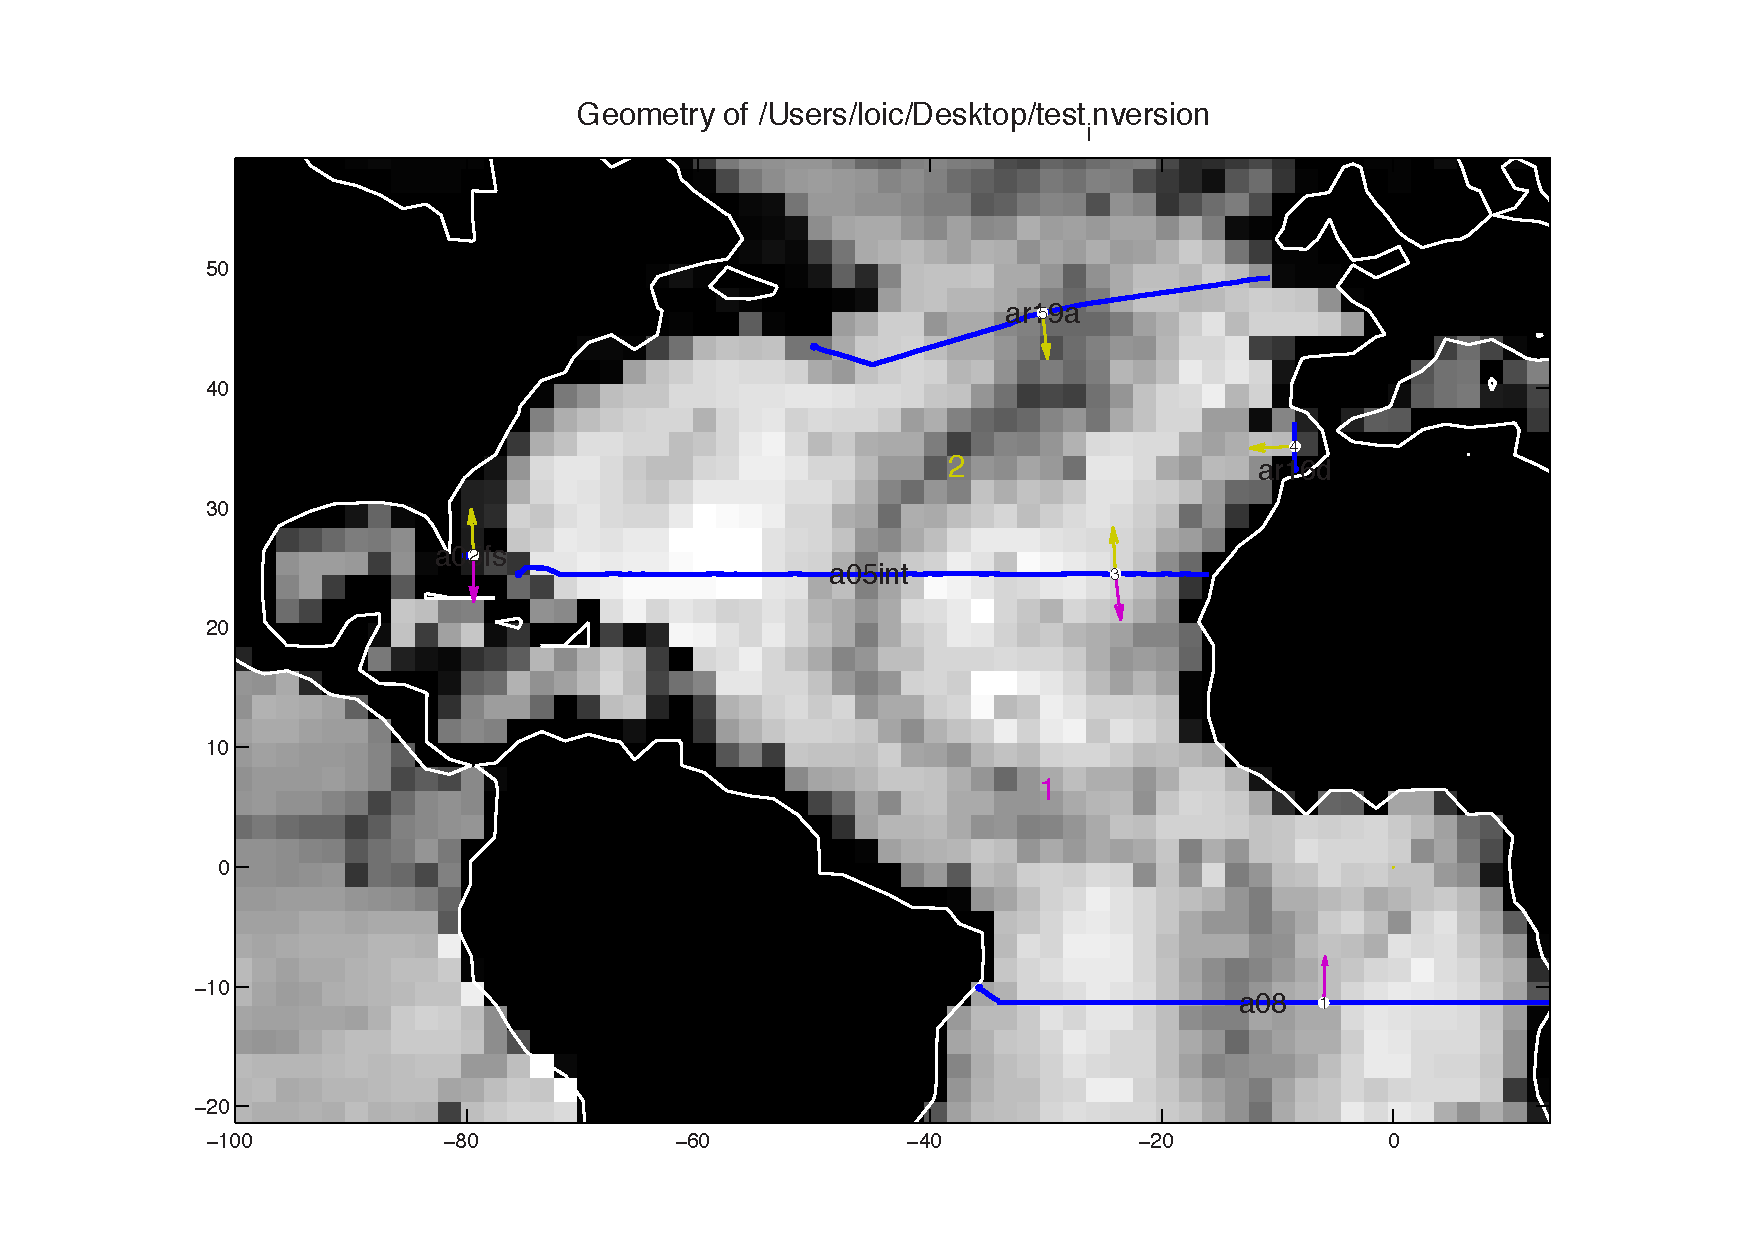
\includegraphics[width=15cm]{fig1.pdf}
\caption{Geometry of the 2 box model in the North Atlantic. This figures is produced by the diagnostic \textit{checkgeo.m}. The box numbers shown for reference.}
\label{fig1}
\end{center}
\end{figure}

%----------------------------------------------------------------------------------------
%	SECTION 4: Constructing the inverse model
%----------------------------------------------------------------------------------------
\section{Inverse model construction using DIABOX}
	\subsection{Formatting the variables in DIABOX format}
	
	At this point, you should know which hydrographic sections and continents will define your closed boxes. You have prepared the sections using \verb"prepctd.m". The sections are run through the step 1 of DIABOX (\verb"dosection.m"). During this step, the CTD sections (2db grid) are used to calculate the variables necessary to construct the inverse model. Inverse models are usually isopycnic models: The fluxes are calculated in density layers and the different variables need to be mapped in density space. We use neutral density \cite{Jackett:1997p370} as our vertical coordinate and a layer of the model is defined by two neutral density contours. \textbf{Note that for now, neutral density is the only density variable allowed by Diabox. This makes it problematic for regions where neutral density is not defined like the Arctic or the Mediterranean Sea}.The code asks you the name of the section you want to process. Diabox is set up so that it will look for the sections in the \verb"test_inversion/section/" subdirectory. Just enter the name of the section:
	
\begin{tabular}{l}
 \verb""\\
\verb">> This gets the raw matlab data file for a section and calculates"\\
\verb"layer thickness and the average value of the tracer in the areas"\\
\verb"of the walls of the box and stores the results in a named file"\\
 \verb""\\
\verb"What raw (section) file name ? a08"\\
 \verb""\\
 
\end{tabular}

	The fluxes in inverse models are calculated as \verb"area * velocities". We calculate the area of the different layers of the model along the section. The area of each grid point of the model is defined as $d_{ii+1}\times h_{j}$, where $d_{ii+1}$ is the distance between two adjacent stations $i$ and $i+1$ and $h_{j}$ is the thickness of the layer $j$ (the pressure (depth) difference between the upper and lower density limit of the layer). For other tracers such as temperature, the transport is the volume transport times the mean temperature of the grid point. In step one, the \verb"Area" for the different tracers are calculated as: 
\begin{center}
\begin{tabular}{ll}
Area($V$) =& $d_{ii+1}\times h_{j}$\\
Area($\Theta$) =& $d_{ii+1}\times h_{j}\times\Theta_{anom}$\\
Area($S$) =& $d_{ii+1}\times h_{j}\times S_{anom}$\\
\end{tabular}
\end{center}
The processed sections are stored in the same directory \verb"/test_inversion/sections" as \verb"a08.mat" in our example. Once all the sections have been ran through step 1, the different components of the inversion are ready to be put together. The following steps will: 

\begin{enumerate}
  \item create the geometry file (\textit{geo.m})
  \item check geometry matrix (\textit{checkgeo.m})
  \item create polygons outlining the boxes (\textit{makeboxcoords.m})
  \item add model-specific constraints (\textit{addconstraints.m})
  \item calculate mean properties (\textit{makemprop.m})
  \item calculate air-sea fluxes on outcropping layers (\textit{makeairsea.m})
\end{enumerate}
	 
	\subsection{Creating the geometry file}
	
	Within the subdirectory for your new box model, you must first edit the file called \textit{geo.m}, which was copied from the main Diabox directory during the execution of the \verb"create_new_inversion" script. This file defines variables  sectfiles, geometry, properties, masssecterror, masstotalerror, and consSILCAT.  Optionally, you may define variables reflevel, rv and vmag.  These optional variables may also be defined in the global file \verb"uniquerefvels.m", and if they are defined there, the entries in \verb"geo.m" will be ignored.  
	
\begin{itemize}
  \item[] \textbf{sectfiles} contains the name of the prepared section files used in your box model.  Note that each entry must have the same number of characters, so extra spaces (which are ignored) are added to the end of many entries.  After executing �geo� in Matlab, you can see how many section files you are using:\verb">> size(sectfiles,1)". 
  \item[] \textbf{geometry} is a matrix of ones, zeros and negative ones. This matrix tells DOBOX how the boxes are bound by the sections.  For more information, see section 3.1.1, �constructing the geometry matrix�.
  \item[] \textbf{reflevel} gives  the thermal wind reference levels (model level numbers) for each section.  This is ignored if it is also specified in \textit{uniquerefvels.m}.
  \item[] \textbf{rv} gives the a priori reference velocities.  This is ignored if also specified in \textit{uniquerefvels.m}.
  \item[] \textbf{vmag} gives the rms magnitude of adjustments to the a priori reference velocities.  This is ignored if also specified in uniquerefvels.m. 
  \item[] \textbf{properties} lists the conserved properties (mass, salinity and potential temperature).
  \item[] \textbf{masssecterror} is the mass error for a section
  \item[] \textbf{masstotalerror} is the net volume imbalance per box, assuming non-synoptic error from section to section are independent.
  \item[] \textbf{consSILCAT}  tells the model to conserve full-depth silicate transport for some of the sections. It is a vector of size equals to the number of sections. The default option is a vector filled with 0s specifying that no silicate constraint should be used on any section. We can add 1 in the rows corresponding to the sections where we want silicate conservation to be applied.
\end{itemize}

		\subsubsection{Constructing the geometry matrix}

Each row represents a box: the number of boxes is \verb"size(geometry,1)".  Each column represents a section file: the number of columns is the number of section files, so you must satisfy \verb"size(sectfiles,1)==size(geometry,2)". 

Each row of geometry (each box of the model) consists of a string of ones, zeros and negative ones. Row one defines how each of the sections bounds box one (the Equatorial Box in our example). The first entry of this row corresponds to section file one, \verb"sectfiles(1,:)".  If box one is not bounded by section one, this entry will be zero. If it is bounded, the value is +1 or �1.  \textbf{The sign convention is identical to DOBOX 4.2 (\cite{Morgan94}, pg. 21): mentally draw an arrow from the first cast in the section file to the final cast. If this arrow is part of a counter-clockwise path around the box, the entry will be +1.  If it is part of a clockwise path around the box, the entry will be �1}. We illustrate with a simple example (Figure \ref{fig2}):

	Box 1 is bound by sections 1, 2 and 3. Because Section 1 runs west-to-east, it is shown as an arrow pointing eastward.  A counter-clockwise circuit around Box 1 runs in the opposite direction, so the appropriate entry in geometry for Section 1, Box 1 is �1 (geometry values shown in parentheses).  For this example, 

\begin{tabular}{ll}
geometry=&     [-1 +1 �1   0;\\
                  &     0   0 +1 +1] ;\\
\end{tabular}


This is an important part of the inversion since it will define the sign of the transport for each box. \textbf{Important}: For very large geometries, such as a global inversion with dozens of sections and boxes, most of the matrix geometry will be zeros.  This is because a section usually defines the edges of at most two boxes (an entry of 1 or -1), and all other row entries for this section�s column will be zero.  In the case of a model with dozens of boxes, hard coding the matrix is undesirable: rows will wrap across lines, negative signs will confuse spacing, and it becomes almost impossible to avoid typographical errors.  Furthermore, you may wish to add or remove a single section � a nightmare with a large, hard-coded geometry matrix!  Instead, create the matrix as in this example:

\begin{tabular}{l}
\verb"%% Now define the geometry."\\
\verb"% See the documentation on how to create the correct geometry file."\\
\verb"% Here is a simple example with 2 boxes in the Atlantic"\\
\verb"% Initialize your geometry file"\\
\verb"geometry=zeros(1,size(sectfiles,1)); bn=1;"\\
\verb"% Fill in 1s for the sections corresponding to the first box."\\
\verb"% CAtl 11S to 24N"\\
\verb"geometry(bn,sectname2sectnum('a05int',sectfiles))=-1;"\\
\verb"geometry(bn,sectname2sectnum('a05fs',sectfiles))=-1;"\\
\verb"geometry(bn,sectname2sectnum('a08',sectfiles))=1;"\\
\verb"% NAtl 24N to 48N"\\
\verb"bn=bn+1;"\\
\verb"geometry(bn,sectname2sectnum('ar19a',sectfiles))=-1;"\\
\verb"geometry(bn,sectname2sectnum('ar16d',sectfiles))=1;"\\
\verb"geometry(bn,sectname2sectnum('a05int',sectfiles))=1;"\\
\verb"geometry(bn,sectname2sectnum('a05fs',sectfiles))=1;"\\
\end{tabular}

This code would be inserted in \verb"geo.m" in place of a hard-coded matrix definition for geometry.  The code is not smart enough to know whether an entry should be 1 or -1, but it�s far preferable to a hard-coded matrix when your model has a dozen boxes!  The routine \verb"sectname2sectnum.m" scans through sectfiles, identifies the row number which contains the section name (the first argument passed to \verb"sectname2sectnum.m"), and returns this row number.  The code above then assigns this to the appropriate column number of geometry, thus avoiding a potential typographical error.

If step 3.1 has been completed successfully, you should be able to \verb"cd" to your model file from within Matlab and enter \verb"geo".  The variables \textit{directory, sectfiles, geometry}, etc. should now be defined in your workspace.

\begin{figure}[h!]
\begin{center}
\includegraphics[width=18cm]{fig2.pdf}
\caption{example geometry: two boxes bounded by two land masses and four sections.}
\label{fig2}
\end{center}
\end{figure}

		\subsubsection{Checking the geometry matrix}

Did you construct the matrix geometry correctly?  It�s easy to make typographical errors, like putting a +1 where you meant -1 or getting that 1 in the wrong column.  First, notice that �interior� sections, those which separate one box from another, and thus bound two boxes,  have a -1 for one box and a +1 for the other.  �Exterior� sections, which define the edge of only one box (like A8 in our example), have only one -1 or +1.  Therefore, if you type �abs(sum(geometry,1)) �, the +1s and -1s should add to zero for interior sections.  Thus, \verb"sectfiles(find(abs(sum(geometry,1))),:)" should list \textbf{only the exterior section files}. Verify this. For our example, these are \textit{a08.mat, ar16d.mat} and \textit{ ar19a.mat}. If the command given above also listed \textit{a05fs.mat} and \textit{a05int.mat}, we would know that there�s a typographical error in geometry: \textit{a05fs} and \textit{a05int} should have the entry -1 for the Subtropical Box and +1 for the Subpolar Box, which would add to 0 and thus not be included in the find.

A more comprehensive check of geometry can be made visually using the script \textit{checkgeo.m}.  Type this:

\begin{tabular}{l}
\verb"clear all; checkgeo('geo');"\\
\end{tabular}

The routine \textit{checkgeo.m} uses the variables in \textit{geo.m} to draw a map of your box model�s geometry.  An example is shown in Fig. \ref{fig1}:

Each section�s casts are plotted as a blue line, with a small black bullet plotted at the first cast.  Superimposed on each section�s cast line is the name of the section file and its section number (column number in \textit{sectfiles}).  Colored arrows point from each section into the box they bound.  Each box is color-coded, with a color randomly chosen.  If \verb"checkgeo.m" happens to choose indistinguishable colors for adjacent boxes, rerun it.

In the example Fig.\ref{fig1}, bounding sections for the North Atlantic subtropical box (box 1) are indicated by magenta arrows.  These sections all have entries of +1 or �1 in �geometry(1,:)�. If a section is showing a magenta arrow, but does not bound box 1, there�s been a typo in the geometry.  For example, if Fig. \ref{fig1} had a magenta arrow on ar19a, then �geometry(1,5)� is �1 or +1, but should be 0.

The direction of the arrow tells you if you�ve entered the correct sign for that section�s entry in geometry.  It should \textbf{point into the box}, as in Fig.\ref{fig1}.  For example, in Fig. \ref{fig1} the two sections bounding box 1 each have a magenta arrow which points into the Subtropical Box� All is well!

	\subsection{Creating polygons defining the boxes (\textit{makeboxcoords.m})}

In the following steps, we will add air-sea fluxes and river runoff to the inversion. We need to know the area of the box and which rivers we need to include. To this effect, box coordinate files, one for each box, must be created using \verb"makeboxcoords.m".  

Enter:  
\begin{tabular}{l}
\verb">>makeboxcoords('geo);"\\
\end{tabular}
The map of your box model appears, similar to the output of \verb"checkgeo.m". In addition, blue stars appear wherever rivers flow into the oceans.  Matlab prompts you to: 

\begin{tabular}{l}
\verb">>Zoom to the desired box (�enter� when done);"\\
\end{tabular}

Using the mouse, click and drag so that box 1 fills the screen. You may wish to click the corner of the figure and enlarge it.  Once box 1, and all the rivers that flow into it, are easily seen on the screen, move the mouse to the Matlab window and hit \verb"enter". Matlab now prompts you to:

\begin{tabular}{l}
\verb">>Mouse-click to define box (�enter� when done);"\\
\end{tabular}

You must now click points which define a closed polygon, enclosing all the oceanic area within box 1, excluding the oceanic area not in the box, and including the rivers flowing into the box. It will also contain parts of the land masses which are not in your oceanic box� this doesn�t matter and is ignored. In the fourbox example, the polygon runs along the path of A8, up the Andes along South and Central America, around the Gulf Coast of North America (and thus includes the Caribbean Sea and Gulf of Mexico in the box), down the Florida Peninsula to A5, along A5 to Africa, and down Africa to the eastern end of A8.  You can start anywhere on this path, and go clockwise or counter-clockwise.  As you click, you are defining the (latitude, longitude) points of a polygon.  Once you�re done, hit \verb"enter" and the polygon is superimposed on the figure. Matlab prompts for 

\begin{tabular}{l}
\verb">>Box number?"\\
\end{tabular}

 Enter \verb"1" for box 1, and a new file appears in your subdirectory boxcoord: \verb"boxcoords1.mat". This file contains the variables \textit{lat, lon} which are also currently in your workspace. The polygon does not have to be perfect, but it should do a reasonable job of following the hydrographic sections where they delineate your box and should not enclose a significant amount of oceanic area which is not in your box.  In this context, �significant� means none of the $0.5^{\circ}$-square grids of ERA should reside within the polygon if the bin is not at least partially within the box, and none of the grids residing within the box should be excluded from the polygon.  

To verify that the boxcoords polygon is successfully identifying water in your box, type:
 
\begin{tabular}{l}
\verb">>checkboxcoords(1)"\\
\end{tabular}  

A map of the region is plotted, and superimposed is a five-by-five degree grid of points which lie within box 1 (the box number is the argument of \verb"checkboxcoords.m"). If this looks good, continue with the rest of your boxes.

\textbf{NOTE: Check carefully boxes which wrap around the dateline. }

 	\subsection{Creating section-specific constraints (\textit{addxconstraints.m})}
	
	%example: a05fs_con.m 
In addition to the main conservation constraints required by inverse models, additional constraints can be build in to reflect our understanding of the circulation. This step is important as it allows to build in extra information in the inverse model to better constrain the inversion. Most of these extra constraints are based on additional information (\textit{e.g} the presence of moorings on a section allows you to calculate the fluxes across this section) and therefore the inclusions of such constraints need to be carefully analyzed (is the constraint reasonable? Is it going to improve the model?).

You can add geometry-dependent constraints to your inversion with the mfile called \verb"add_xconstraints.m". A template is copied in the relevant directory (in the model geometry subdirectory) during the inversion set up. This file contains two sets of commands that can be applied to all the boxes. First of all, it can impose conservation for the entire domain (the transport across the outer sections of the domain is conserved). Secondly, it can impose full-depth silicate conservation for each section. Finally it contains the names of mfiles containing section specific constraints. For example, in the test inversion, it calls three mfiles: \verb"a05fs_con;", \verb"ar16d_con;" and \verb"a08_con;". Each of those files contains a series of commands:

\begin{tabular}{l}
\verb"%------------------------------------------------------"\\
\verb"sectnum=sectname2sectnum('arch');"\\
\verb"statnum=[];"\\
\verb"propnum=1;"\\
\verb"boxnum=3;"\\
\verb"ayernum=nlayers+1;"\\
\verb"fluxvalue=0.8e6;"\\
\verb"fluxerror=masssecterror(sectnum)^2;"\\
\verb"addcon;"\\
\verb"%------------------------------------------------------"\\
\end{tabular}\\

\textbf{sectnum}: the section number.  You can use \textit{sectname2sectnum.m} to get this.  If the constraint is to be applied to more than one section (example: 0 Sv across two sections), \textit{sectnum} can be a vector of section numbers.  

\textbf{statnum}:  the cast (station) numbers.  For example, you may wish to impose a western boundary current transport to stations 1-25 of a section running west-to-east.  Enter the station numbers as they appear in the prepared Matlab files.  If \verb"statum=[]" has been entered, the constraint will be applied to all casts in the section(s).  NOTE: the code assumes that there is only one section in \textit{sectnum} if station numbers are specified in \textit{statnum}.  I have no idea what would happen if you specify station numbers and multiple section numbers.

\textbf{propnum}: the property number, specified in the section files.  By DOBOX convention, 1=mass, 2=salt and 3=heat.

\textbf{boxnum}: the box number.  Only one value can be given.

\textbf{layernum}: the layer number(s).  Set to \verb"nlayers+1" to apply the constraint to all the layers, i.e. make the constraint a top-to-bottom constraint.

\textbf{fluxvalue}: the value you wish to constraint the transport.  As currently constructed, DIABOX assumes the units are SI.  Volume transports are m$^{3}$ s$^{-1}$, so 5Sv should be entered as \verb"5e6".

Once all the parameters have been set, \verb"addcon.m" creates the extra constraint terms and add them to the corresponding inversion variables (A, b and R$_{nn}$).

	\subsection{Calculate mean properties (\textit{makemprop.m})}
 
Diapycnal fluxes of mass, heat and salt (other tracers too) require a knowledge of the mean tracer value on the isopycnal through which the fluxes occur as well as an estimation of the area of the isopycnal in the box (Eq. \ref{conservation_2}). Therefore, we need to use a climatology in order to obtain a knowledge of the vertical structure of the temperature and salinity field in the box and calculate the correct area, temperature and salinity of the isopycnals used in the box. \verb"makemprop.m" does this calculation.

We use a climatology. For now, only the WOCE Global Hydrography Climatology (WGHC, \cite{Gouretski2004}). This is a relatively old climatology but offers the advantage to interpolate data onto isopycnal coordinates rather than depth coordinates. More recent climatologies could be implemented too. \verb"makemprop.m" reads the climatology, interpolate the data onto isopycnals. Then, it isolates the data points located only in the box and calculate the mean area of the ocean interface and of all the layers as well as the mean (and standard deviation) pressure, temperature and salinity over each isopycnal.

	\subsection{Calculate air-sea fluxes on outcropping layers (\textit{makeairsea.m})}

	Air-sea heat (M$_{\theta}$)  and mass(M$_{v}$)  flux as well as the associated water mass transformation (F$_{v}$) can be calculated by integrating the air-sea freshwater flux (\emph{Q}) and the air-sea net heat flux (\emph{H}) derived from air-sea reanalysis and ocean climatologies:

\begin{eqnarray}\label{surfmixing}
M_{\theta} &=& \int_{T}dt\int_{A}\frac{H}{C_{p}\rho}dA,\\
M_{v} &=& \int_{T}dt\int_{A}\frac{-Q}dA,\\
F_{v} &=& \int_{T}dt\int_{A_{\Delta}}(\frac{1}{\Delta \rho}(\frac{\alpha H}{C_{p}} - \rho \beta Q S))dA,
\end{eqnarray}

where $\Delta \rho$ is the potential density interval centered at $\rho$ over which the flux is calculated; $C_{p}$ is the specific heat capacity of the ocean; $\alpha$ and $\beta$ are the thermal expansion and haline contraction coefficients, respectively; $A_{\Delta}$ is the outcropping area of the density interval $\Delta \rho$; and \emph{A} is the outcropping area of a layer of mean potential density $\rho$.  $F_{v}$ is the diapycnal volume flux across a layer interface (positive toward lighter density) arising from changes in buoyancy induced by net heat and freshwater exchanges between the ocean and the atmosphere. The $F_{v}$ and $M_{\Theta}$ terms are weighted by the square root of the prior uncertainty. Note that the net volume gain M$_{v}$ is far smaller than the uncertainties due to the baroclinic variability in the upper ocean and is often neglected \citep{ganachaud03b}.

	In the previous version of DIABOX, there was a choice of several climatologies. Now, only ERA-Interim is used as it is usually thought to be the least bad of climatologies in the high latitudes of the Southern Hemisphere. The main routine is \verb"makeairsea.m" which calculates both the formation/transformation of water masses at the surface due to air-sea forcing and the Ekman transport. An example of ERA-Interim net heat flux is shown in Figure \ref{fig4}

\begin{figure}[h!]
\begin{center}
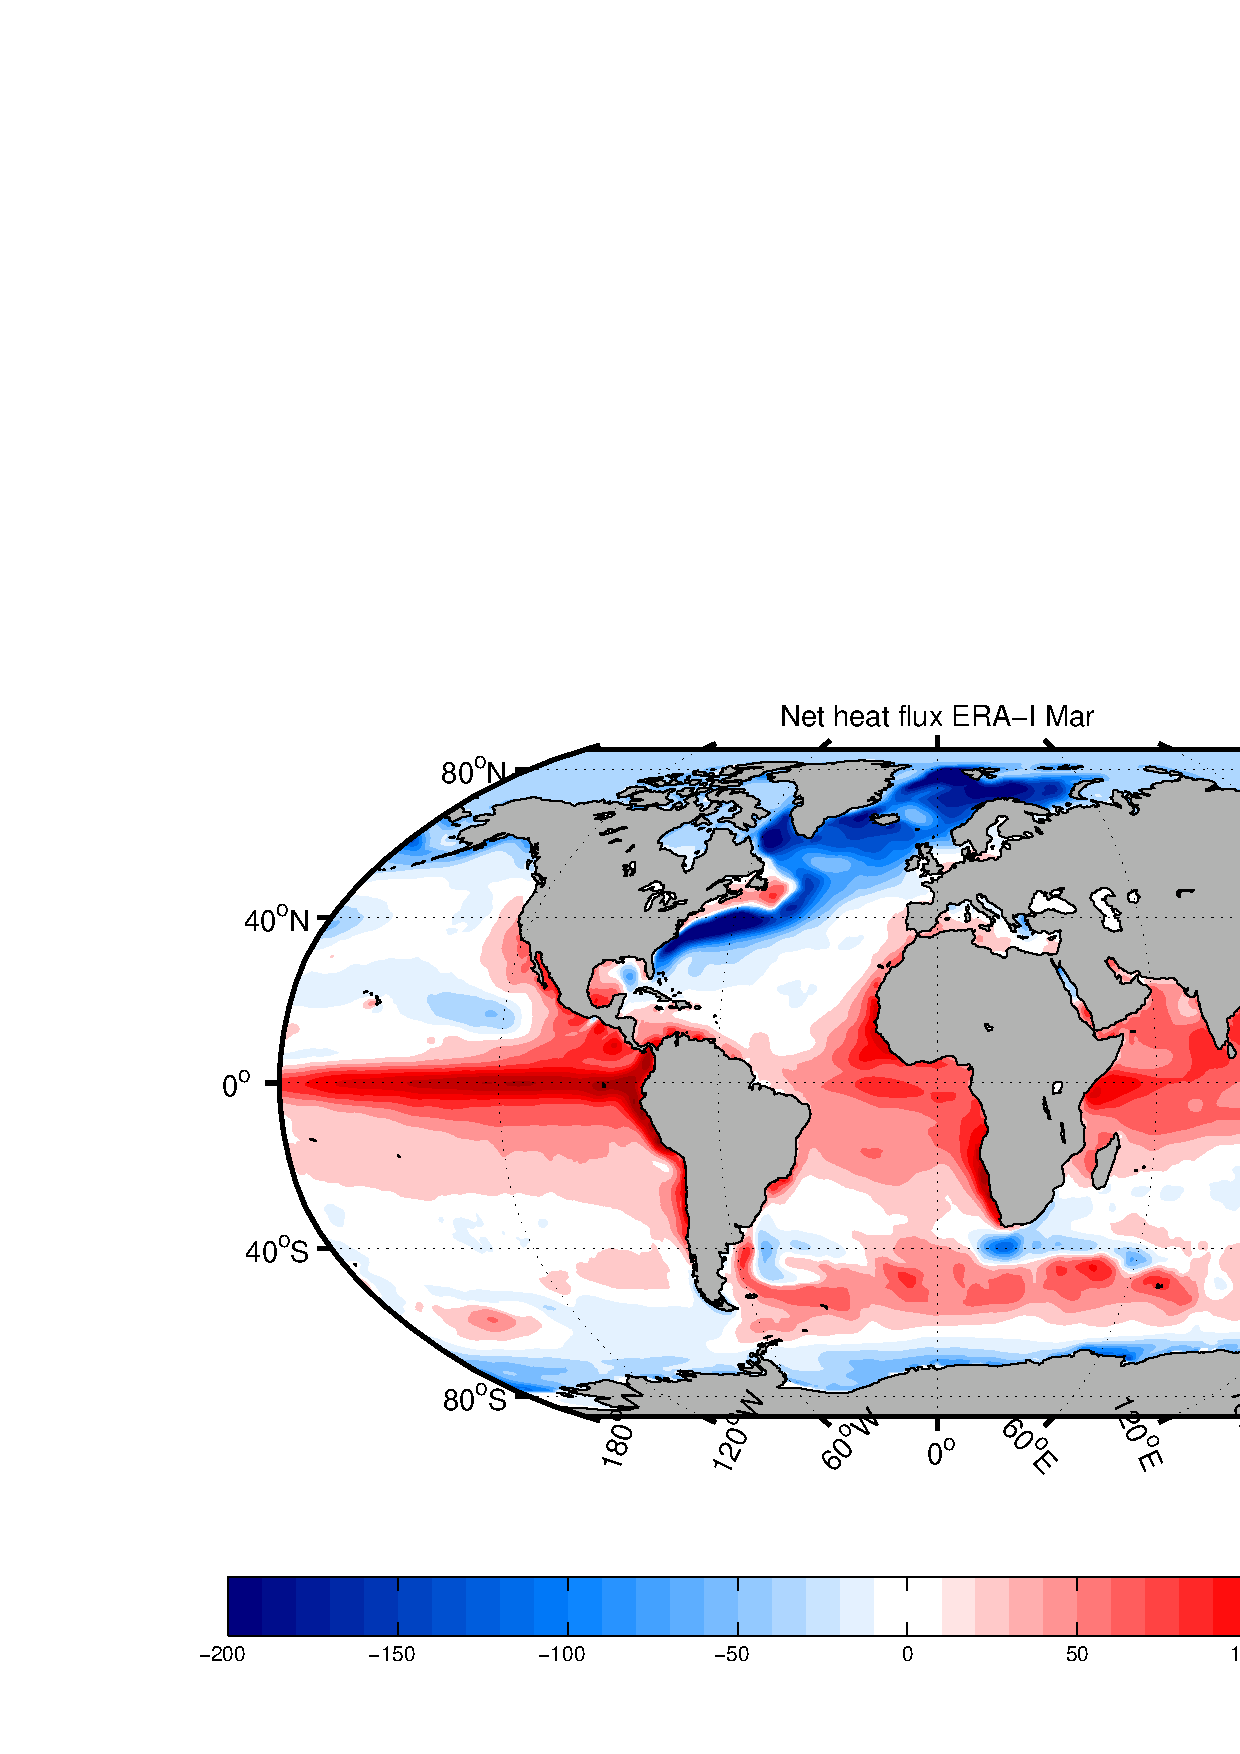
\includegraphics[width=18cm]{fig4.pdf}
\caption{Monthly mean average (1979-2012) of net heat flux for March (W m$^{-2}$)}
\label{fig4}
\end{center}
\end{figure}

	The netcdf files for ERA interim are stored in the \verb"Diabox_v2.0/Anc_data/ERA" directory. Right now, they span the 1979-2012 time period and will need to be updated. The time period for the reanalysis can be specified in \verb"makeairsea.m" using the  \textit{year} variable. We can use one year, several years or climatological values calculated from ERA-Interim. All the air-sea fluxes are then vectorized. This tends to make the calculation faster than with 3-D matrices. Each variable has a size of [12,nx*ny]: One row for each month of the year, and nx*ny data points where nx is the number of longitudes and ny the number of latitudes. If we load more than one year of data, then all the years will be concatenated so that with 2 years of data, each variable will have a size of [24,nx*ny]. The function \verb"loaderayear.m" loads the data. 
	
	Care must be taken when dealing with reanalysis data because not all variables are the same. ERA-Interim has 3 types of data: analyzed (the observations corrected by the model), forecast and accumulated forecast. Most fluxes (precipitation, air-sea heat fluxes...) are accumulated forecasts. No monthly means of daily means are available for download even if the web site states that it is on their to do list. To calculate monthly means of daily means, a work around is to download the 2 synoptic monthly means (time 00, step 12 and time 12, step 12), to add them together and then divide by the forecast period (24 hours). All of this can be found in the ERA-Interim FAQs.

	In the main \verb"makeairsea.m" routine, the mfile \verb"calcflux.m" calculates the density, salt and heat flux due to air-sea forcing and the Ekman transport. In order to assign the air-sea fluxes and Ekman transport to the right density layer of the model, one needs to get surface density distribution as a function of the month. Ideally we would like monthly SST and SSS fields over the same time period than the air-sea climatology. ERA-Interim provides SST data than can be used but they do not provide any SSS. Instead, we use the recently developped MIMOC climatology based on available hydrographic data including ARGO floats. MIMOC provides 12 monthly climatological fields of SST, SST and density as well as values of temperature, salinity and pressure of the mixed layer which is useful for the Ekman calculation. Air-sea heat and mass fluxes, water mass transformation and Ekman fluxes are calculated for each box and are saved in individual \verb".mat" files \verb"airsea1.mat, airsea2.mat" \ldots where the number corresponds to the box number.
%
%\begin{figure}[h]
%\begin{center}
%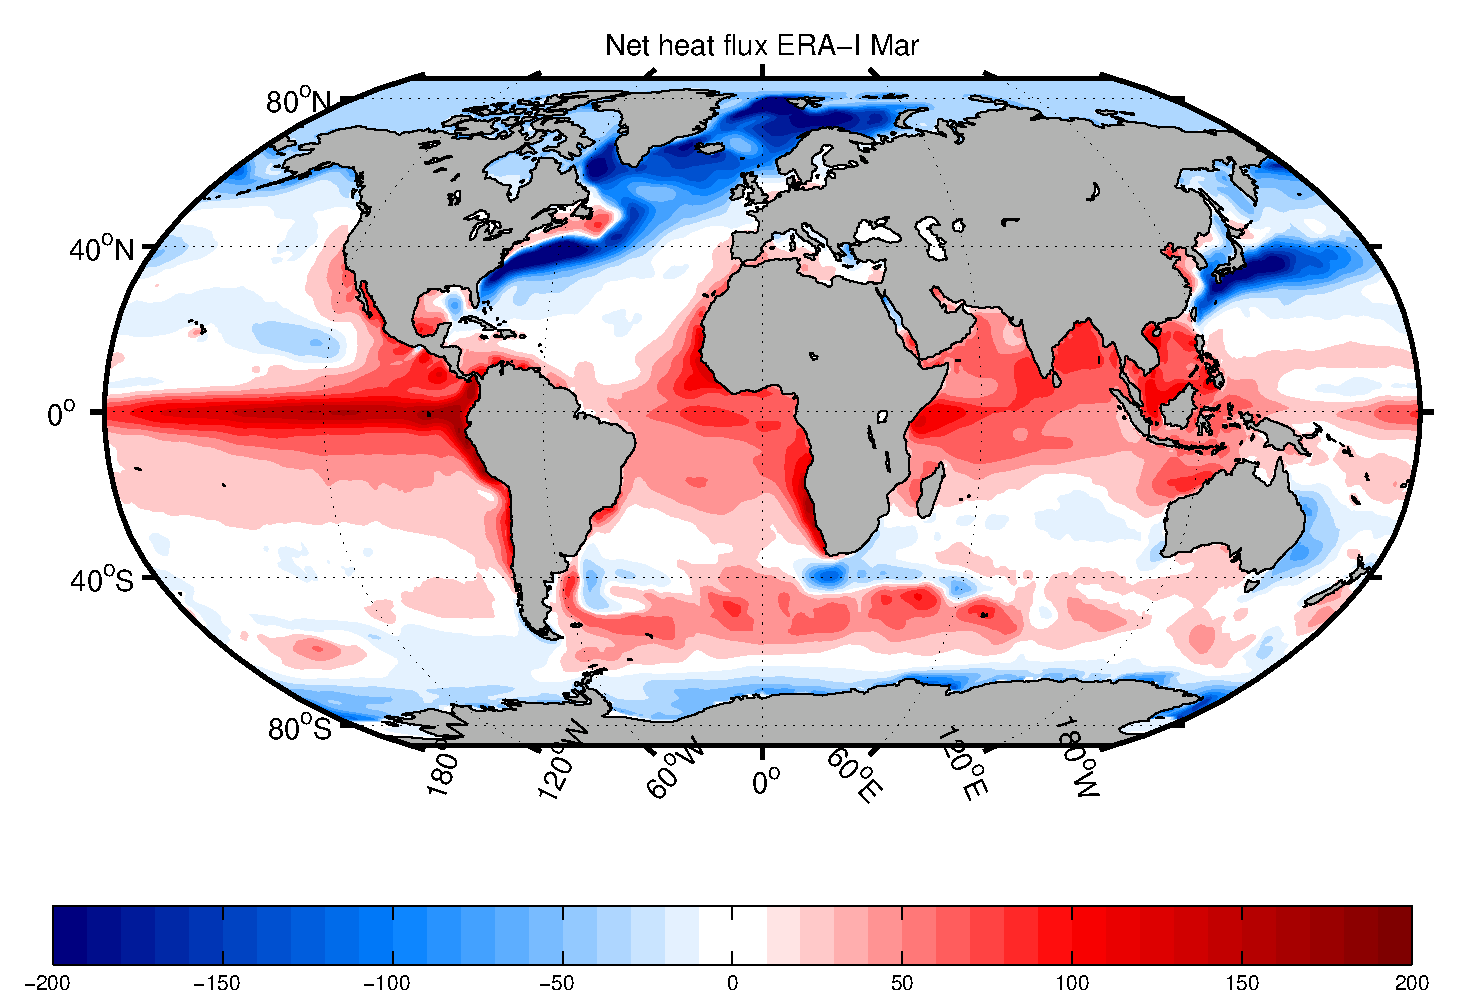
\includegraphics[width=1\textwidth]{fig4.eps} \label{fig4}% Include the image placeholder.png
%\caption{Climatological net air sea heat fluxes calculated for the ERA-interim period (1979-2012) for the month of March.}
%\end{center}
%\end{figure}

	\subsection{Creating the \textit{a priori} reference velocities (refvels.m)}
	
	In the geometry file \verb"geo.m", default choices for the \textit{a priori} reference levels and velocities are made. This default option sets for each section the reference level (\verb"reflevel") to the Deepest Common Level (DCL), the reference velocities (\verb"rv") to 0 m s$^{-1}$), equivalent to setting the \textit{a priori} barotropic component of the thermal wind equation to 0, and the error on the velocities (\verb"Vmag") to 0.01 m s$^{-1}$.
	
	In the mfile \verb"refvels.m", these default choices are used to construct the reference velocities vector (\verb"RV") for each section:
	\begin{center}
	\begin{tabular}{l}
\verb"% after \\ : \hline or \cline{col1-col2} \cline{col3-col4} ..."\\
\verb"geo;"\\
\verb"% loop through sections;"\\
\verb"for i=1:size(geometry,2);"\\
\verb""\\
\verb"	sectname=sectfiles(i,:);"\\
\verb"	eval(['load ',sectname,' lon']);"\\
\verb"	RV=rv(i)*ones(length(lon)-1,1)';"\\
\verb"	Vmag=vmag(i)*ones(length(lon)-1,1)';"\\
\verb"	q=find(sectname=='/');"\\
\verb"	sectname(1:last(q))=[];"\\
\verb"	q=find(sectname=='.');"\\
\verb"	sectname=sectname(1:q-1);"\\
\verb"	rvfilename=['refvel_',sectname];"\\
\verb"	eval(['save ',rvfilename,' RV Vmag']);"\\
\verb""\\
\verb"end;"\\
\end{tabular}
\end{center}
	
This default choice might not be appropriate for all sections. For example, in the Southern Ocean, the Antarctic Circumpolar Current is an equivalent-barotropic geostrophic current made of several bottom-reaching fronts, implying that the whole water column moves eastward and that therefore, the bottom velocities might not be null. In the South Atlantic, the Antarctic Bottom Water is going north at the bottom whereas the North Atlantic Deep Water is going south. This implies that the bottom velocities might not be 0 and that there might be a depth further up in the water column at the interface between AABW and NADW where the velocities is 0. As a consequence, \textit{a priori} reference velocities and reference levels need to be specified in order to reflect our knowledge of the circulation. The choice of reference levels and velocities is done on a section by section basis in the mfile \verb"uniquerefvels.m". Here is an example where for one section, the reference velocities are adjusted independently in different part of the sections:

\begin{center}
\begin{tabular}{l}
\verb"%%%%%%%%%%%%%%%%%%%%%%%%%%%%%%%%%%%%%%%%%"\\
\verb"% a08 (11 deg. S)."\\
\verb"%"\\
\verb"% Initial reference levels from Speer, Holfort,"\\
\verb"%	Reynaud and Siedler (1996)."\\
\verb"sect='a08.mat';"\\
\verb"i=sectname2sectnum(sect,sectfiles);"\\
\verb"if (length(i))"\\
\verb""\\
\verb"  refp=3900;"\\
\verb"  eval(['load ',sectdir,'/a08_raw bin_press surf_press']);"\\
\verb"  d=(refp-nanmean(surf_press')').^2;"\\
\verb"  reflevel(i)=find(d==min(d));"\\
\verb""\\
\verb"  Vmag=defVmag(sectfiles(i,:),reflevel(i),.01,100,.3);"\\
\verb"  RV=rv(i)*ones(length(Vmag),1)';"\\
\verb""\\
\verb"  % shift reference level to isobaric surfaces"\\
\verb"  % (ASSUMES BOTTOM REFERENCE LEVEL)"\\
\verb"  reflevel(i)=length(glevels);  % must be set to bottom"\\
\verb"                                % for isobaric code to work!"\\
\verb"  eval(['load ',sectdir,'/a08_raw bin_press lon binPair_vel']);"\\           
\verb"  lon=lon(1:length(lon)-1)+diff(lon)/2;"\\
\verb"  for j=1:length(lon);"\\
\verb"    q=find(isfinite(binPair_vel(:,j)));"\\
\verb"    binPair_vel(:,j)=binPair_vel(:,j)- ..."\\
\verb"	binPair_vel(last(q),j);"\\
\verb" end;"\\
\end{tabular}
\end{center}

\begin{center}
\begin{tabular}{l}
\verb""\\
\verb"  % shift ref level to 1100m west of 35.5W"\\
\verb"  q=find(bin_press==1100);"\\
\verb"  q2=find(lon<=-35.5);"\\
\verb"  RV(q2)=RV(q2)-binPair_vel(q,q2);"\\
\verb"  q=find(isnan(RV(q2)));RV(q2(q))=0;"\\
\verb"  %RV(3)=-.2886;"\\
\verb""\\
\verb"  % shift ref level to 3800m between 35.5W and 17.67W"\\
\verb"  % (Brazil Basin)  (stations 4:6 stay bottom-referenced)"\\
\verb"  q=find(bin_press==3800);"\\
\verb"  q2=find(lon>=-35.5 & lon<=-17.67);"\\
\verb" RV(q2)=RV(q2)-binPair_vel(q,q2);"\\
\verb"  q=find(isnan(RV(q2)));RV(q2(q))=0;"\\
\verb""\\
\verb"  % shift ref level to 2400m between 17.67W and 10.17W (MAR)"\\
\verb"  q=find(bin_press==2400);"\\
\verb"  q2=find(lon>=-17.67 & lon<=-10.17);"\\
\verb"  RV(q2)=RV(q2)-binPair_vel(q,q2);"\\
\verb"  q=find(isnan(RV(q2)));RV(q2(q))=0;"\\
\verb""\\
\verb"  % shift ref level to 4000m east of 10.17W (Angola Basin)"\\
\verb"  q=find(bin_press==4000);"\\
\verb"  q2=find(lon>=-10.17);"\\
\verb"  RV(q2)=RV(q2)-binPair_vel(q,q2);"\\
\verb"  q=find(isnan(RV(q2)));RV(q2(q))=0;"\\
\verb""\\
\verb"  % uniform shift to balance Ekman (9.71Sv south)"\\
\verb"  RV=RV-1.23e-4;"\\
\verb""\\
\verb"  clear binPair_vel lon bin_press q q2"\\
\verb""\\
\verb"  rvfilename=['refvel_',sect];"\\
\verb"  eval(['save ',rvfilename,' RV Vmag']);"\\
\verb""\\
\verb"end;"\\
\verb""\\
\verb"%%%%%%%%%%%%%%%%"\\
\end{tabular}
\end{center}

One of the limitation of DOBOX and DIABOX is the inability to specify several reference levels for a given box. If the DCL is chosen for a section of box 1, then the DCL will be used as the reference level for all the sections. This implies that for all the sections, we need to specify in \textit{RV} the velocity at the DCL. 

%----------------------------------------------------------------------------------------
%	SECTION 4
%----------------------------------------------------------------------------------------
\section{Setting up the matrices and inverting}

	\subsection{Constructing the matrices}
Now all the initial steps have been completed and the different components of the inverse model are ready to be assembled. In the original DOBOX software, all the different steps necessary to construct the matrix were manual, necessitating a user input. In DIABOX, most of the steps have been automated which should save some time and potentially avoid errors caused by loading the wrong files. The DIABOX interface looks like:
\begin{center}
\begin{tabular}{l}
\verb"***************************************************************"\\
\verb"**            DIABOX Version 2.0                              **"\\
\verb"***************************************************************"\\
\verb" 						"\\
\verb"----- BOX MENU (0) : Model Choices -----"\\
\verb" 						"\\
\verb"      1) Prepare raw Section file for diabox      "\\
\verb"			                "\\
\verb"      2) Lhs      - Define geometry, build Abase 	"\\
\verb"      3) Rhs      - Set reflevel, build bbase 	"\\
\verb"      4) Build    - Define interior diapycnal mixing, build A & b"\\
\verb" 				          "\\
\verb"      5) Solve via Gauss-Markov estimation"\\
\verb" "\\ 				
\verb"      0) Matlab       -    Return to MATLAB "\\		
\verb""\\  							
\verb" Select a menu number: {2} "\\
\verb""\\
\end{tabular}
\end{center}

\textbf{Option 1} has already been described previously.

\textbf{Option 2} loads the geometry file \verb"geo.m" and construct the matrix \verb"A" using the function \verb"build_a.m". The matrix A has dimensions of (nproperties*nboxes) by (nstationpairs+nextra unknowns).

\textbf{Option 3} loads the different reference velocity files and calculate the matrix \textit{D} containing the \textit{a priori} transports. In the original DOBOX software, the different reference velocity mat files and the name of the file in which the referenced-geostrophic velocities is saved had to be entered manually. In DIABOX, this step is automated (\verb"rhs_menu.m). The matrix D is constructed and the geostrophic velocities are saved in \verb"getfluxes.m".

\textbf{Option 4} Load and append the extra unknowns (extra columns) to the matrix \verb"A". As the model is built, only the interior diapycnal fluxes are built in during option 4. The diapycnal fluxes are initialized in the routine called \textit{xcolint.m} and they are saved in a variable called \verb"Xcols". Later on in the code (in \verb"gauss.m"), air-sea fluxes will be added too. In \verb"xcolint.m", for each box, the mean area, potential temperature and salinity of each layer interface calculated in \verb"makemprop.m" are loaded and diagonal matrices are constructed. For each box, an Xcols matrix with dimensions [nproperties*nsurfs,length(levels)*nproperties] filled with 0s and 2 diagonals with areas on the diagonal and -area on the next lower diagonal. Finally, the different \verb"Xcols" are then concatenated in one \verb"Xcols" variable saved in \verb"Xcols.mat" alongside a variable \verb"XCW" where the uncertainties on the diapycnal fluxes will be stored.

At this point, most of the matrix \verb"A" and the \verb"a priori" residuals \verb"b" have been calculated. The inversion is saved in a variable called \verb"readyforgauss.mat". After option 4, there is no need to run the main dobox menu. The base of the inverse mode is constructed and saved. This final steps (adding air-sea fluxes, setting the weights, solving Eq. \ref{matrix_form} using the Gauss-Markov estimation are done in the routine \verb"gauss.m".

\textbf{Option 4}  runs the final  routine \textit{gauss.m}.

	\subsection{The master routine \textit{gauss.m}}
	
	This is where the magic happens. The different mfiles used are described in the section.
	
		\subsubsection{defindices}

This function identifies the indices corresponding to the different components of A, x and b in Eq. \ref{matrix_form} using the data structure pointers (see the original DOBOX manual, pp. 24). We define the indices for the different unknowns of the system (columns):
\begin{itemize}
\item indv = Indices for ref. velocity
\item indw = Indices for the diapycnal velocities w
\item indF = Indices for air-sea forcing corrections (tacked on after w* terms)
\item indE = Indices for Ekman transport corrections"
\end{itemize}

For the different equations (rows):

\begin{itemize}
\item indb = (row) indices for property fluxes
\end{itemize}

Here are a few examples:
\begin{itemize}
\item x(indv(i)) = reference velocity at stn. pair i
\item x(indw(i,j,k)) =  diapycnal velocity at level i of property j, box k.
\item b(indb(i,j,k)) = layer i flux of property j, box k.(i=nlayers+1 for vertical integral)
\end{itemize}

Finally, the function also returns the mean property for each layer in the different boxes (e.g. meanprop(i,j,k) = mean value of property j at level i, in box k). These indices are very useful to identify the correct positions in the matrix. This is particularly useful for inversions with multiple boxes when the number of rows and unknowns quickly become overwhelming. 

		\subsubsection{getXcol}
The diapycnal velocities have been added to the inversion with the \verb"get_diapvel" function. Now we refine the additional terms of the inverse model. Note that this function should be updated if one want to new terms to the inversion. As it stands, this routine:
\begin{itemize}
\item Adjusts the diapycnal velocities for some bugs
\item Take into account the advection across isopycnals for properties other than mass (PT, S).
\item Load the air-sea fluxes and Ekman transport calculated by the \verb"makeairsea.m" file 
\end{itemize}
%----------------------------------------------------------------------------------------
%	SECTION 5
%----------------------------------------------------------------------------------------
\section{Plotting and interpreting results}



%----------------------------------------------------------------------------------------
%	BIBLIOGRAPHY
%----------------------------------------------------------------------------------------
\clearpage
\bibliographystyle{../../../templates_journals/AGU/agu08}

\bibliography{diaboxbib}

%----------------------------------------------------------------------------------------


\end{document}